%!TEX TS-program = pdflatexmk

% Copyright (c) 2018 - 2022, Martin Scheidt (ISC license)
% Permission to use, copy, modify, and/or distribute this file for any purpose with or without fee is hereby granted, provided that the above copyright notice and this permission notice appear in all copies.

\documentclass[border=2]{standalone}

\usepackage[dev]{tikz-trackschematic}

\begin{document}
  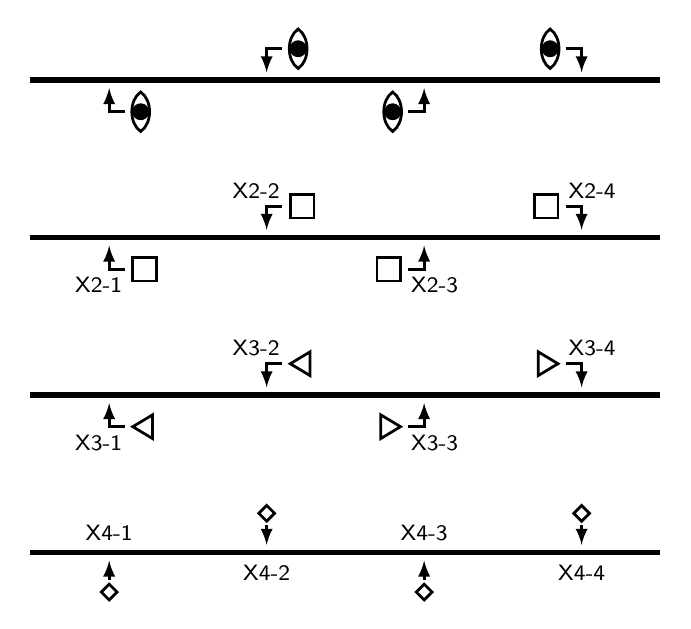
\begin{tikzpicture}
  
    \foreach \i in {1,2,...,4}{% base coordinate
      \coordinate (A\i) at ($(0,0) + 2*(0,-\i)$);% base coordinate
      \coordinate (B\i) at ($(8,0) + 2*(0,-\i)$);% base coordinate
    }

    \foreach \i in {1,2,...,4}{% draw main tracks on base coordinate
      \maintrack (A\i) --   (B\i);
    }

    \foreach \i in {1,2,...,4}{% coordinates for testing symbols
      \coordinate (X\i-1) at ($(1,0) + 2*(0,-\i)$);
      \coordinate (X\i-2) at ($(3,0) + 2*(0,-\i)$);
      \coordinate (X\i-3) at ($(5,0) + 2*(0,-\i)$);
      \coordinate (X\i-4) at ($(7,0) + 2*(0,-\i)$);
    }

    \viewpoint[forward ] at (X1-1);
    \viewpoint[forward ,position=left] at (X1-2);
    \viewpoint[backward,position=left] at (X1-3);
    \viewpoint[backward] at (X1-4);

    \movementauthority[forward ] at (X2-1) label (X2-1);
    \movementauthority[forward ,position=left] at (X2-2) label (X2-2);
    \movementauthority[backward,position=left] at (X2-3) label (X2-3);
    \movementauthority[backward] at (X2-4) label (X2-4);

    \brakingpoint[forward ] at (X3-1) label (X3-1);
    \brakingpoint[forward ,position=left] at (X3-2) label (X3-2);
    \brakingpoint[backward,position=left] at (X3-3) label (X3-3);
    \brakingpoint[backward] at (X3-4) label (X3-4);

    \dangerpoint[forward] at (X4-1) label (X4-1);
    \dangerpoint[forward ,position=left] at (X4-2) label (X4-2);
    \dangerpoint[backward,position=left] at (X4-3) label (X4-3);
    \dangerpoint[backward] at (X4-4) label (X4-4);

  \end{tikzpicture}
\end{document}